%%%%%%%%%%%%%%%%%%%%%%% file template.tex %%%%%%%%%%%%%%%%%%%%%%%%%
%
% This is a general template file for the LaTeX package SVJour3
% for Springer journals.          Springer Heidelberg 2010/09/16
%
% Copy it to a new file with a new name and use it as the basis
% for your article. Delete % signs as needed.
%
% This template includes a few options for different layouts and
% content for various journals. Please consult a previous issue of
% your journal as needed.
%
%%%%%%%%%%%%%%%%%%%%%%%%%%%%%%%%%%%%%%%%%%%%%%%%%%%%%%%%%%%%%%%%%%%
%
% First comes an example EPS file -- just ignore it and
% proceed on the \documentclass line
% your LaTeX will extract the file if required
\begin{filecontents*}{example.eps}
%!PS-Adobe-3.0 EPSF-3.0
%%BoundingBox: 19 19 221 221
%%CreationDate: Mon Sep 29 1997
%%Creator: programmed by hand (JK)
%%EndComments
gsave
newpath
  20 20 moveto
  20 220 lineto
  220 220 lineto
  220 20 lineto
closepath
2 setlinewidth
gsave
  .4 setgray fill
grestore
stroke
grestore
\end{filecontents*}
%
\RequirePackage{fix-cm}
%
%\documentclass{svjour3}                     % onecolumn (standard format)
%\documentclass[smallcondensed]{svjour3}     % onecolumn (ditto)
\documentclass[smallextended]{svjour3}       % onecolumn (second format)
%\documentclass[twocolumn]{svjour3}          % twocolumn
%
\smartqed  % flush right qed marks, e.g. at end of proof
%
%
% \usepackage{mathptmx}      % use Times fonts if available on your TeX system
%
% insert here the call for the packages your document requires
%\usepackage{latexsym}
%\usepackage{longtable}

\usepackage{xfrac}   
\usepackage{lineno}  
\usepackage{graphicx}
\usepackage{color}
\usepackage{multirow}
\usepackage{array}
\usepackage{setspace} 
\usepackage{makecell}
\usepackage{amsmath}

%DEFINED BY NELSON NAZZICARI: defining this command so we can have 
% wrapping (p) columns horizontally centered in tables
\newcolumntype{C}[1]{>{\centering\let\newline\\\arraybackslash\hspace{0pt}}m{#1}}

%since we only have supplementary materials in this document
\renewcommand{\figurename}{Suppl. Fig.}
\renewcommand{\tablename}{Suppl. Table}


%ADDED FOR PEER REVIEW: these commands to be deleted in the final version
\linenumbers
\doublespacing %this command to be removed

% Insert the name of "your journal" with
\journalname{Molecular Breeding}
%
\begin{document}

\title{
Marker imputation efficiency for Genotyping-By-Sequencing data of crop species with and without a reference genome 
\thanks{Nelson Nazzicari and Filippo Biscarini contributed equally to the work \\
Corresponding author: Nelson Nazzicari \email{nelson.nazzicari@entecra.it}}
}
%\subtitle{Do you have a subtitle?\\ If so, write it here}

% if too long for running head
\titlerunning{Imputation efficiency for GBS data with and without the reference genome}        

\author{Nelson Nazzicari \and
  Filippo Biscarini  \and
  Paolo Cozzi \and
  E. Charles Brummer \and
  Paolo Annicchiarico
}

\authorrunning{Nazzicari, Biscarini et al.} % if too long for running head

\institute{
    N. Nazzicari, P. Annicchiarico \at Council for Agricultural Research and Economics (CRA) Research Centre for Fodder Crops and Dairy Productions, Lodi (Italy)
\and
    F. Biscarini, P. Cozzi \at Dipartimento di Bioinformatica, Fondazione Parco Tecnologico Padano, Lodi (Italy)
\and
    E.C. Brummer \at University of California, Plant Sciences Department, Davis, CA (USA)
}


\date{Received:  / Accepted:}
% The correct dates will be entered by the editor

\maketitle

\graphicspath{{./figures/}}
\section{Supplementary material}
\label{sec:supplementary_material}

\subsection{SNP calling thresholds}
\label{sec:SNP_calling_thresholds}
Genotype calling can incur in two types of error, namely a heterozygote wrongly identified as homozigote ($HET \rightarrow HOM$) and the reverse case ($HOM \rightarrow HET$). 
Under the simplifying hypothesis of absence of sequencing errors and homogeneous sequencing quality, it is possible to estimate error rates for a tetraploid genome using the following formula:

\begin{equation}
\begin{cases}
0.75^{N_h} + 0.25^{N_h} & HET_{3-1} \rightarrow HOM \\ 
2 \times 0.5^{N_h}      & HET_{2-2} \rightarrow HOM \\ 
0                       & HOM \rightarrow HET
\end{cases}
\end{equation}

Where $N_h$ is the minimum number of reads required to label a stack of aligning reads as heterozygote. The discussed case of $N_h = 11$ brings to a total expected $HET \rightarrow HOM$ error rate of 4.22\%.\\
The hypothesis mentioned above greatly simplyfies the real case (e.g. $HOM \rightarrow HET$ errors can not happen, since a homozigote will always produce 100\% of reads of the same type). When accounting sequencing errors and reads quality a term for $HOM \rightarrow HET$ appears, due to reads sequenced as the wrong allele. In the presented study we thus applied a threshold of 4 required reads per stack to call a homozigote to minimize this kind of error.

\subsection{Supplementary figures}
\label{sec:supplementary_figures}

\begin{figure}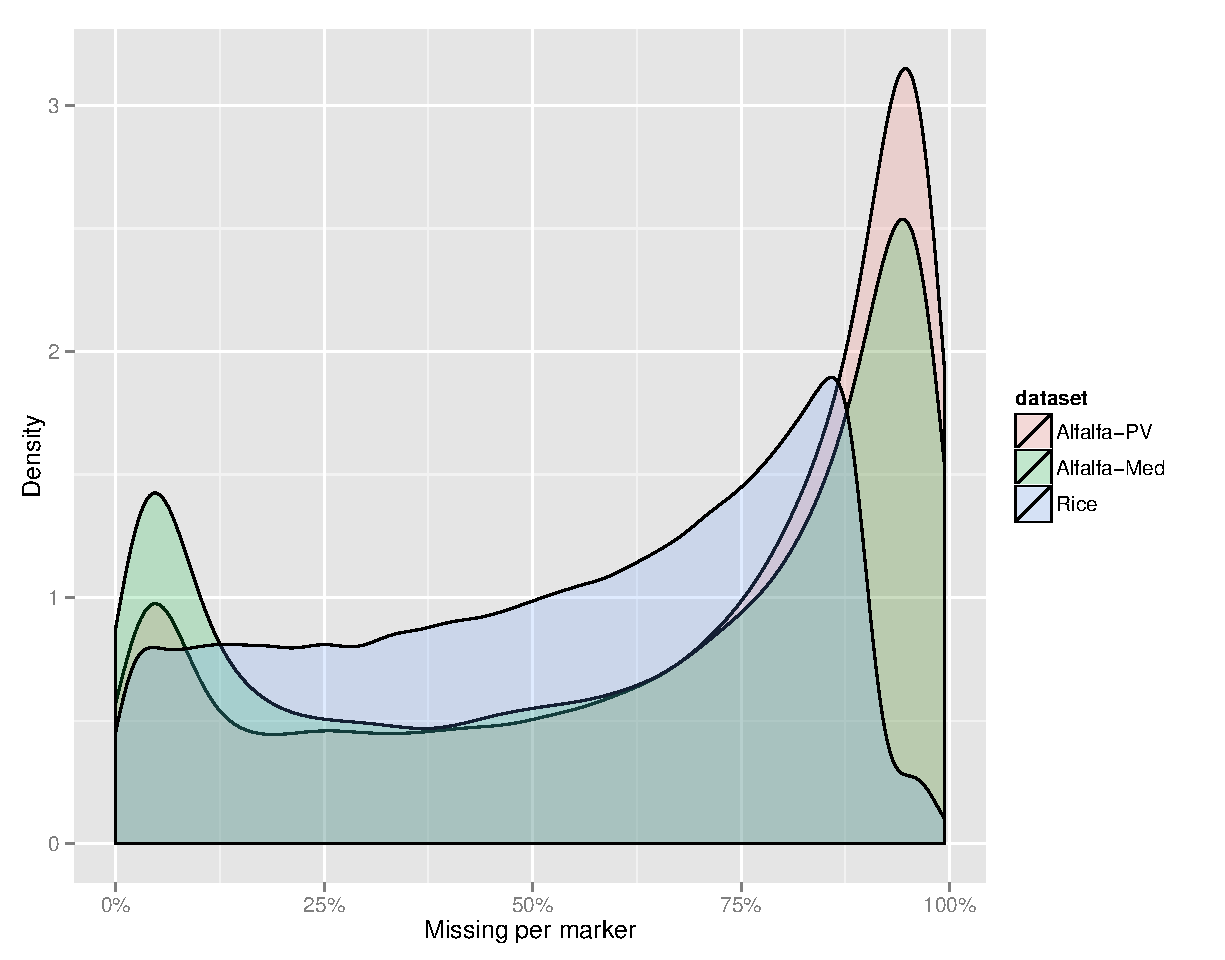
\includegraphics[width=0.95\textwidth]{SupplFig01_miss_per_marker.pdf}
\caption{Distribution of missings-per-marker rates in the three datasets. This is a
density plot, so all curves delimit the same unitary area.}
\end{figure}

\begin{figure}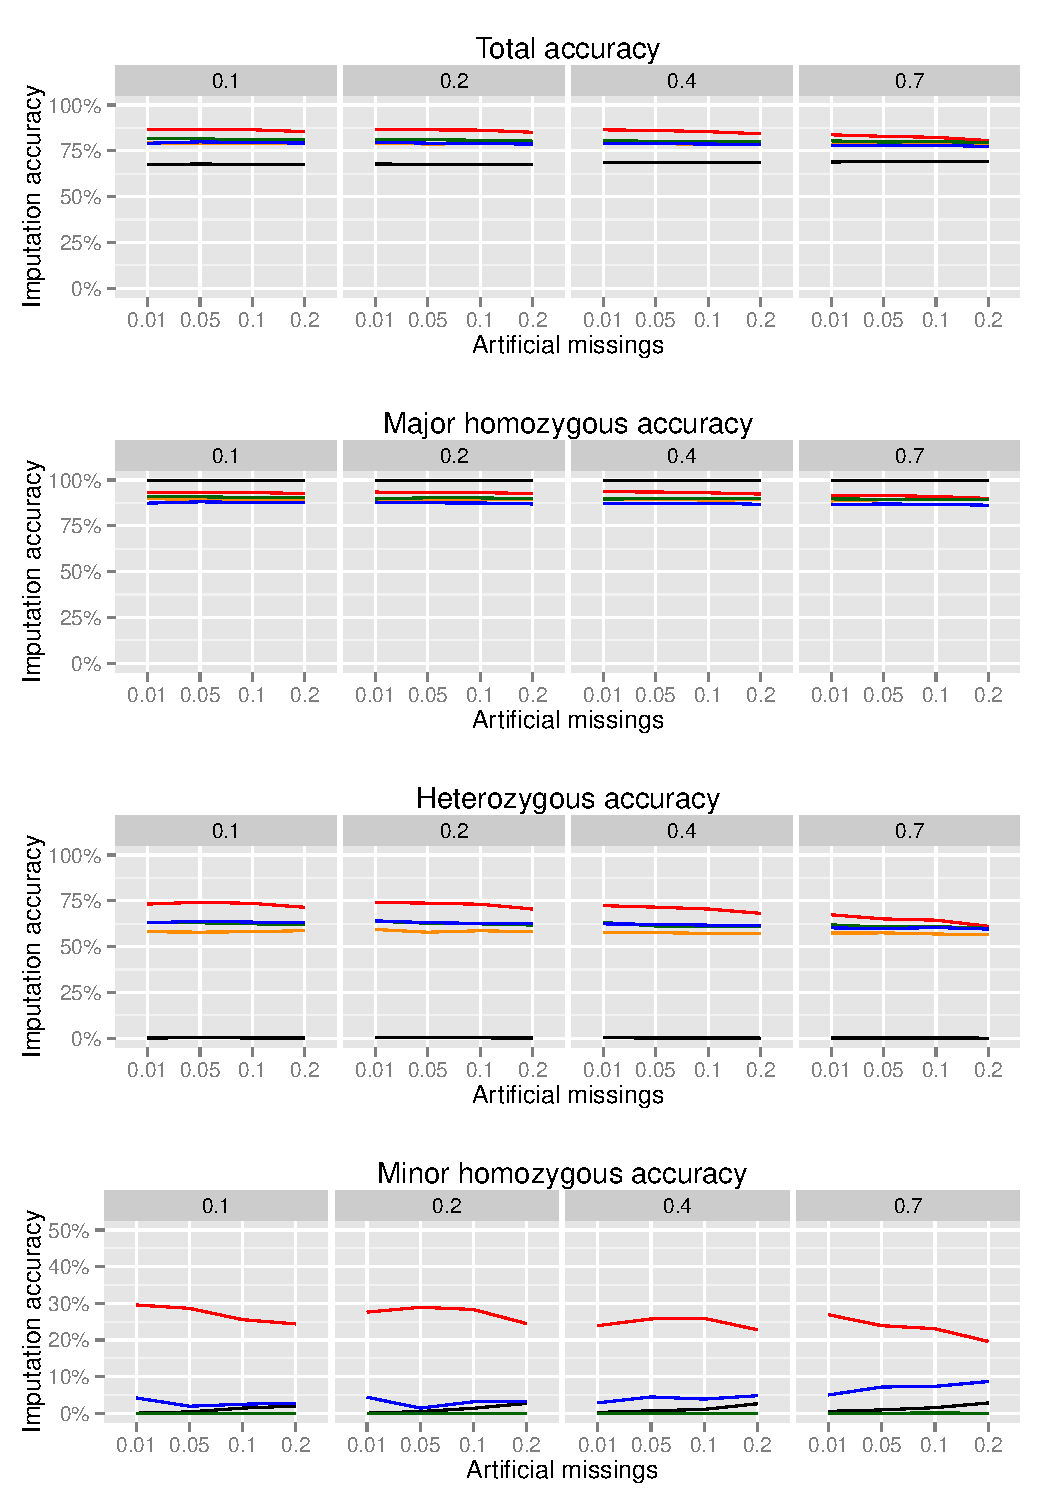
\includegraphics[width=0.95\textwidth]{SupplFig02_Alfalfa-Med.pdf}\caption{
imputation accuracies overall, for the major homozygous genotype (AA), for heterozygotes (AB), and for the minor homozygous genotype (BB) in datasets consisting of
10\%, 20\%, 40\% and 70\% allowed missing data per locus (boxes) with 1\%, 5\%, 10\% and 20\%
additional missing values artificially introduced (x-axis) for alfalfa population Alfalfa-Med.
Lines colors represent the five imputation algorithms: MNI
(orange), KNNI (red), SVDI (blue), RFI (green) and Beagle (black)}\end{figure}
\begin{figure}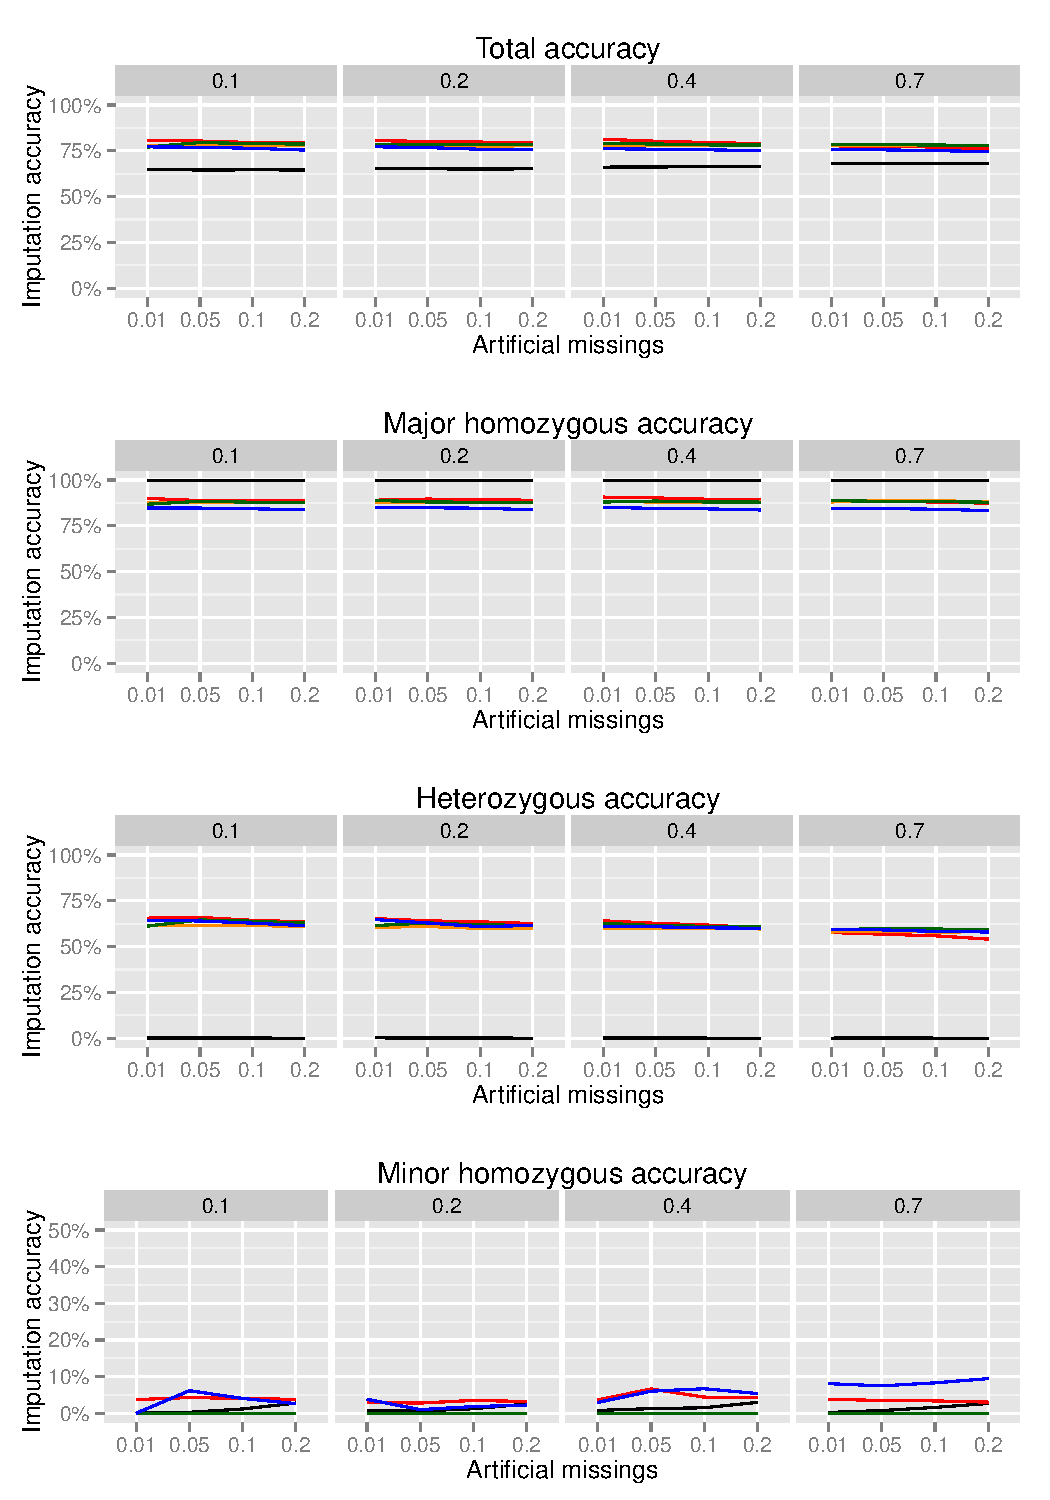
\includegraphics[width=0.95\textwidth]{SupplFig03_Alfalfa-PV.pdf}\caption{
imputation accuracies overall, for the major homozygous genotype (AA), for heterozygotes (AB), and for the minor homozygous genotype (BB) in datasets consisting of
10\%, 20\%, 40\% and 70\% allowed missing data per locus (boxes) with 1\%, 5\%, 10\% and 20\%
additional missing values artificially introduced (x-axis) for alfalfa population Alfalfa-PV.
Lines colors represent the five imputation algorithms: MNI
(orange), KNNI (red), SVDI (blue), RFI (green) and Beagle (black)}\end{figure}
\begin{figure}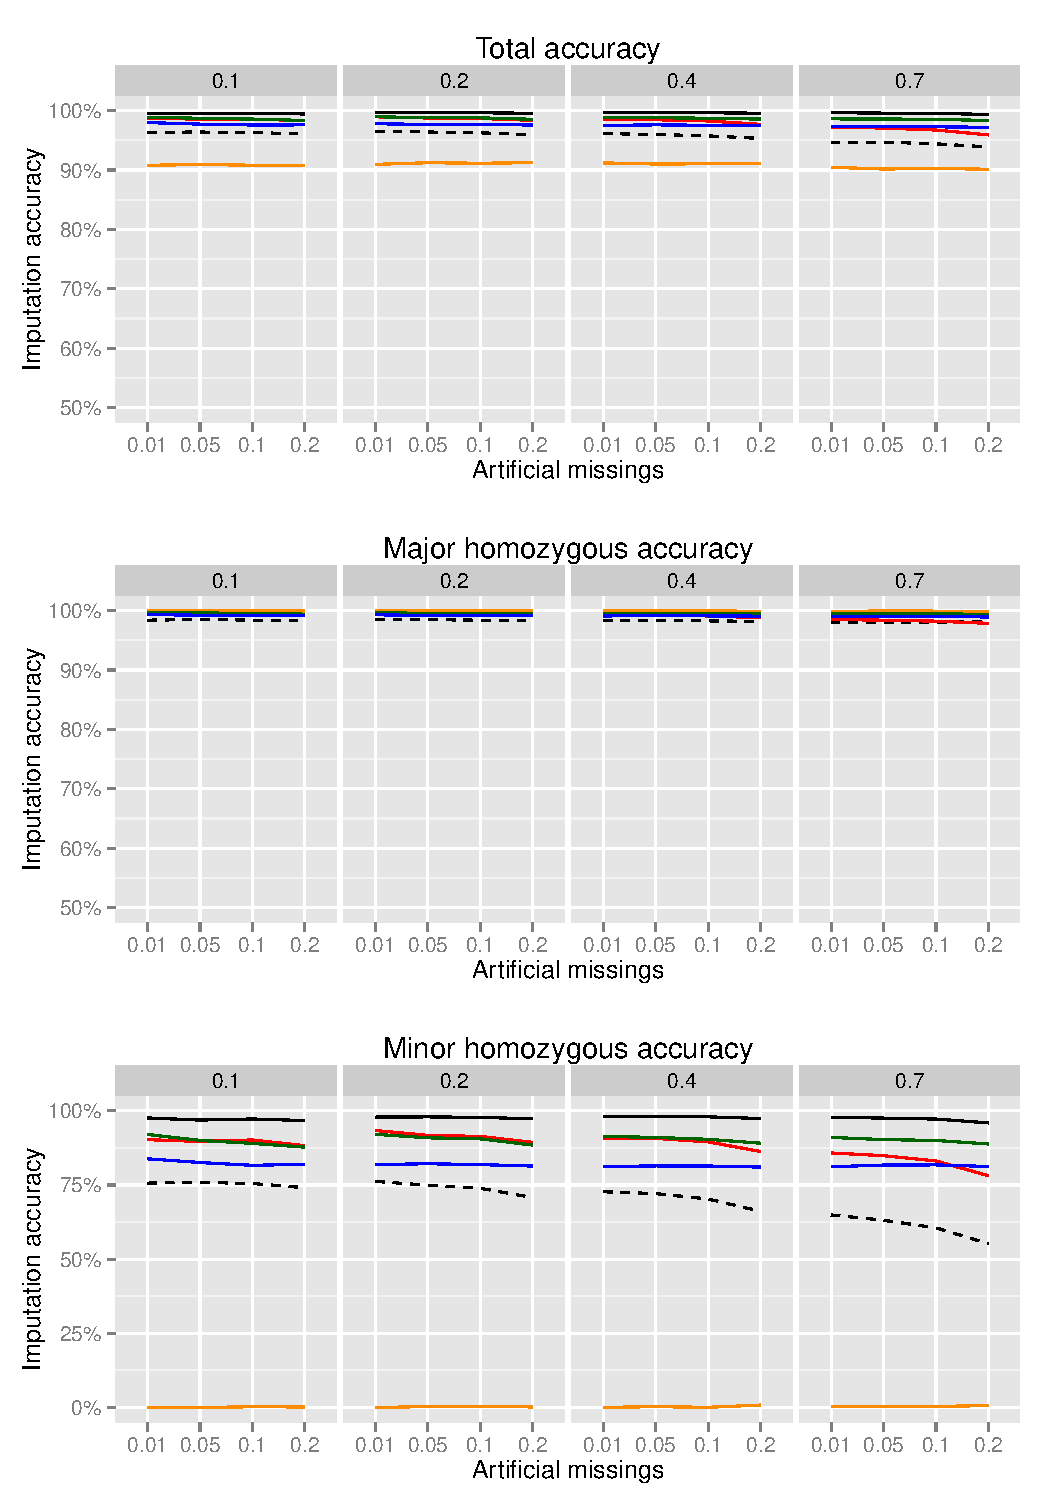
\includegraphics[width=0.95\textwidth]{SupplFig04_Rice-chrom-1.pdf}\caption{
imputation accuracies overall, for the major homozygous genotype (AA) and for the minor homozygous genotype (BB) in datasets consisting of
10\%, 20\%, 40\% and 70\% allowed missing data per locus (boxes) with 1\%, 5\%, 10\% and 20\%
additional missing values artificially introduced (x-axis) for rice chromosome 1 data.
Lines colors represent the five imputation algorithms: MNI
(orange), KNNI (red), SVDI (blue), RFI (green) and Beagle (black)}\end{figure}
\begin{figure}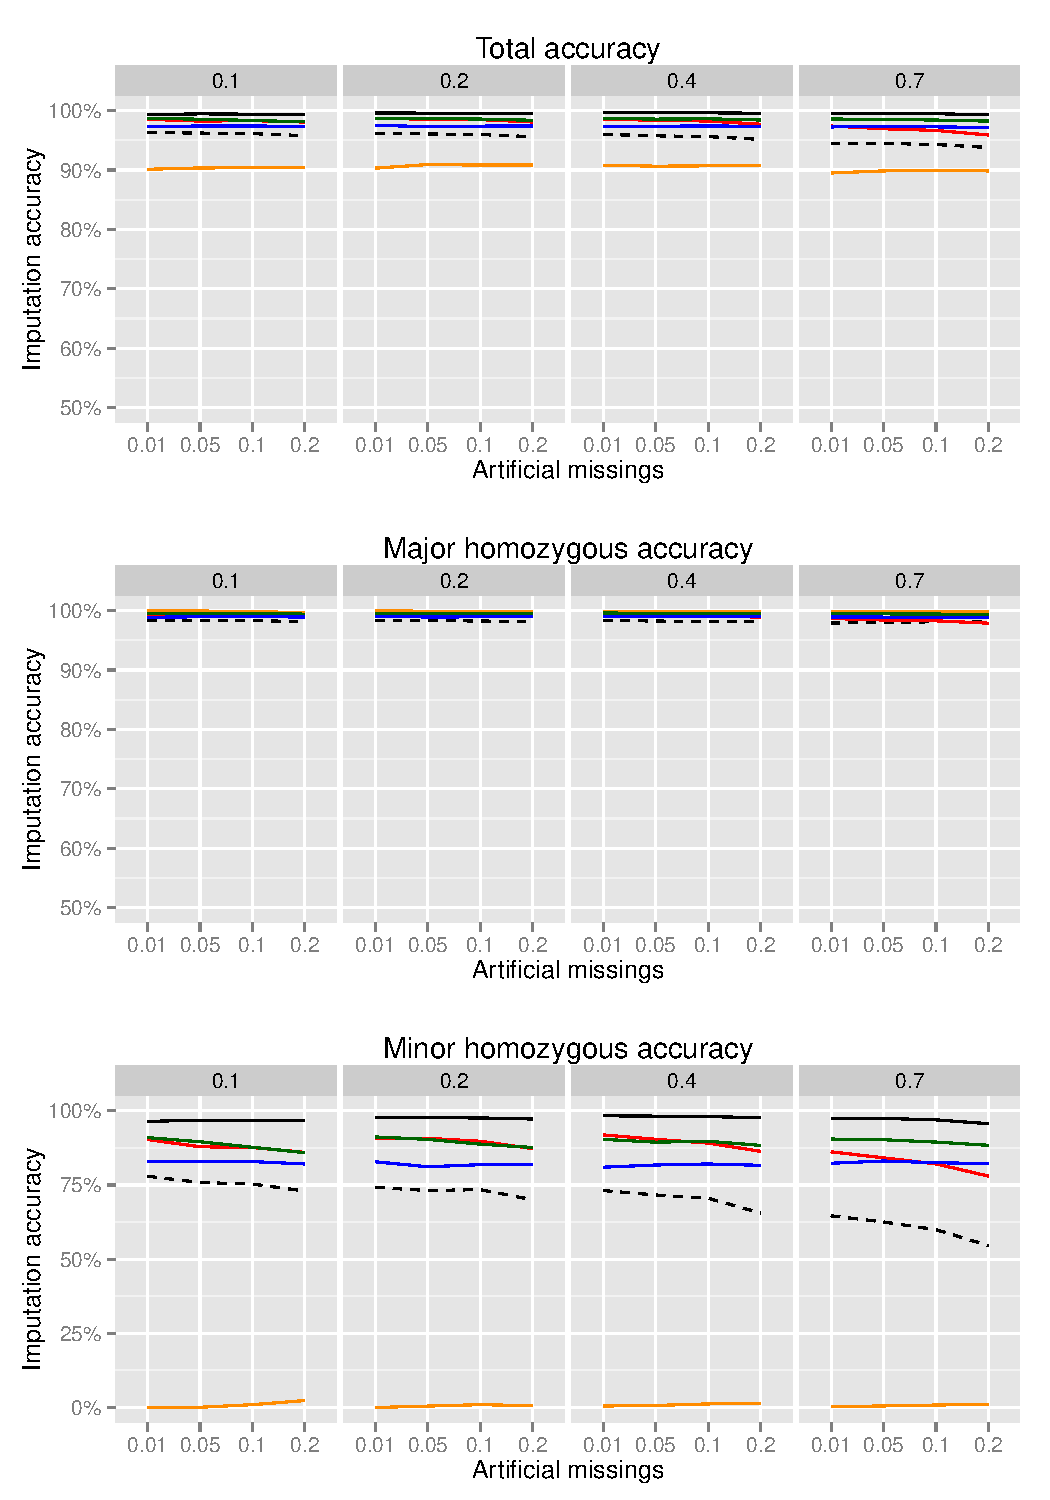
\includegraphics[width=0.95\textwidth]{SupplFig05_Rice-chrom-2.pdf}\caption{
imputation accuracies overall, for the major homozygous genotype (AA) and for the minor homozygous genotype (BB) in datasets consisting of
10\%, 20\%, 40\% and 70\% allowed missing data per locus (boxes) with 1\%, 5\%, 10\% and 20\%
additional missing values artificially introduced (x-axis) for rice chromosome 2 data.
Lines colors represent the five imputation algorithms: MNI
(orange), KNNI (red), SVDI (blue), RFI (green) and Beagle (black)}\end{figure}
\begin{figure}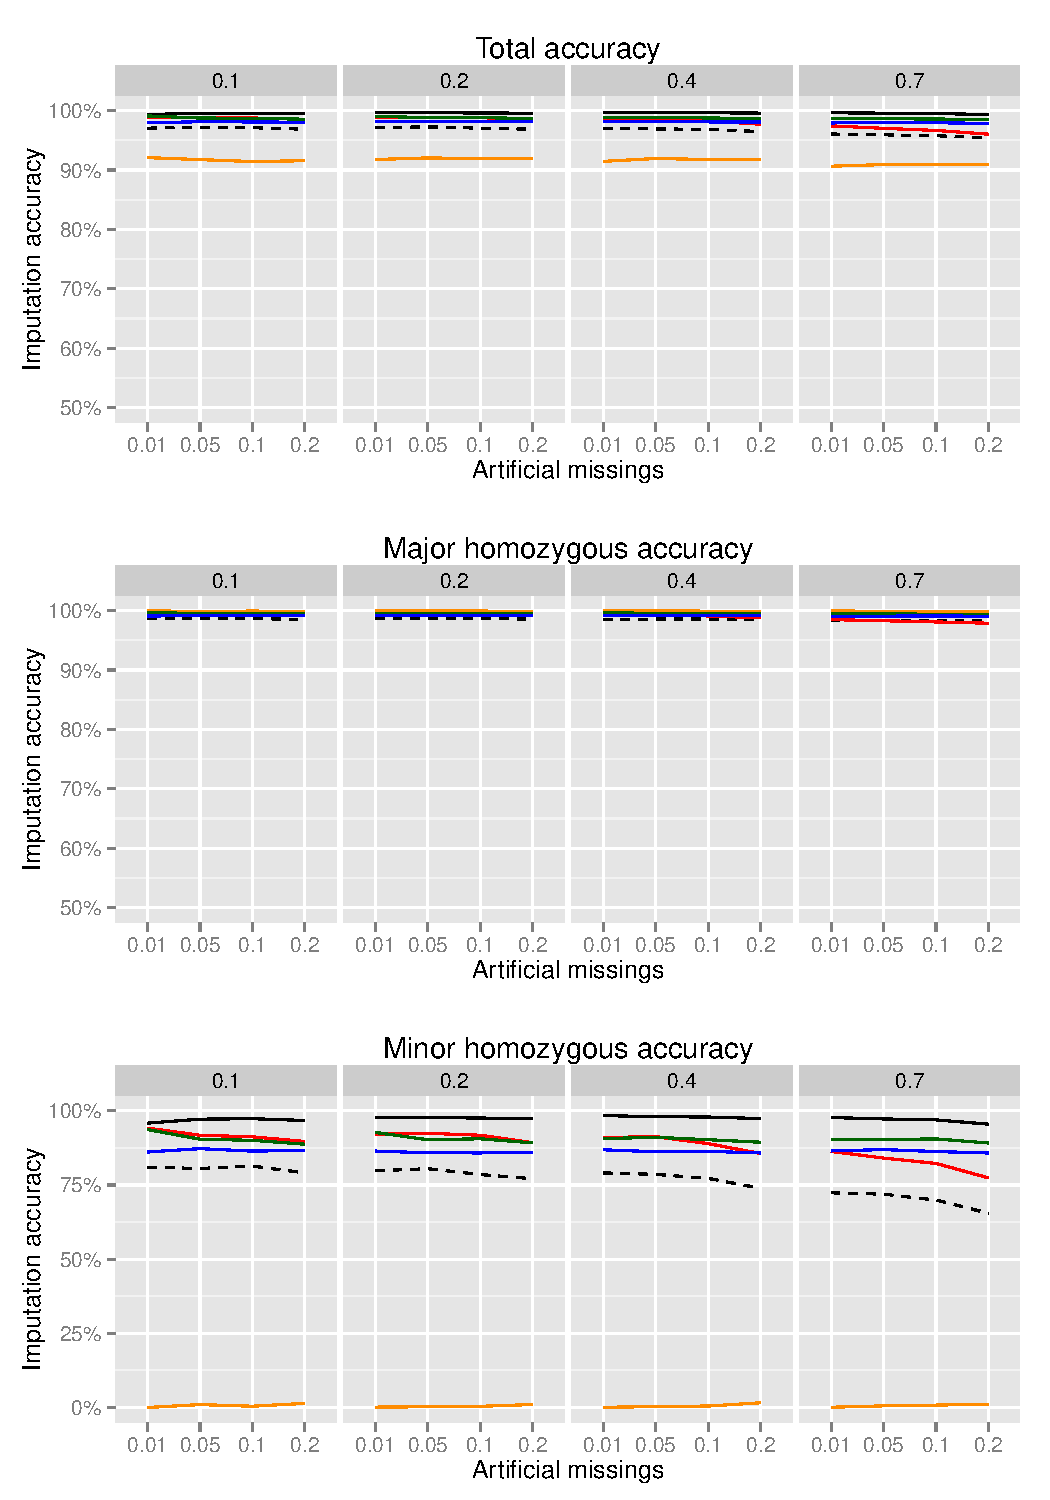
\includegraphics[width=0.95\textwidth]{SupplFig06_Rice-chrom-3.pdf}\caption{
imputation accuracies overall, for the major homozygous genotype (AA) and for the minor homozygous genotype (BB) in datasets consisting of
10\%, 20\%, 40\% and 70\% allowed missing data per locus (boxes) with 1\%, 5\%, 10\% and 20\%
additional missing values artificially introduced (x-axis) for rice chromosome 3 data.
Lines colors represent the five imputation algorithms: MNI
(orange), KNNI (red), SVDI (blue), RFI (green) and Beagle (black)}\end{figure}
\begin{figure}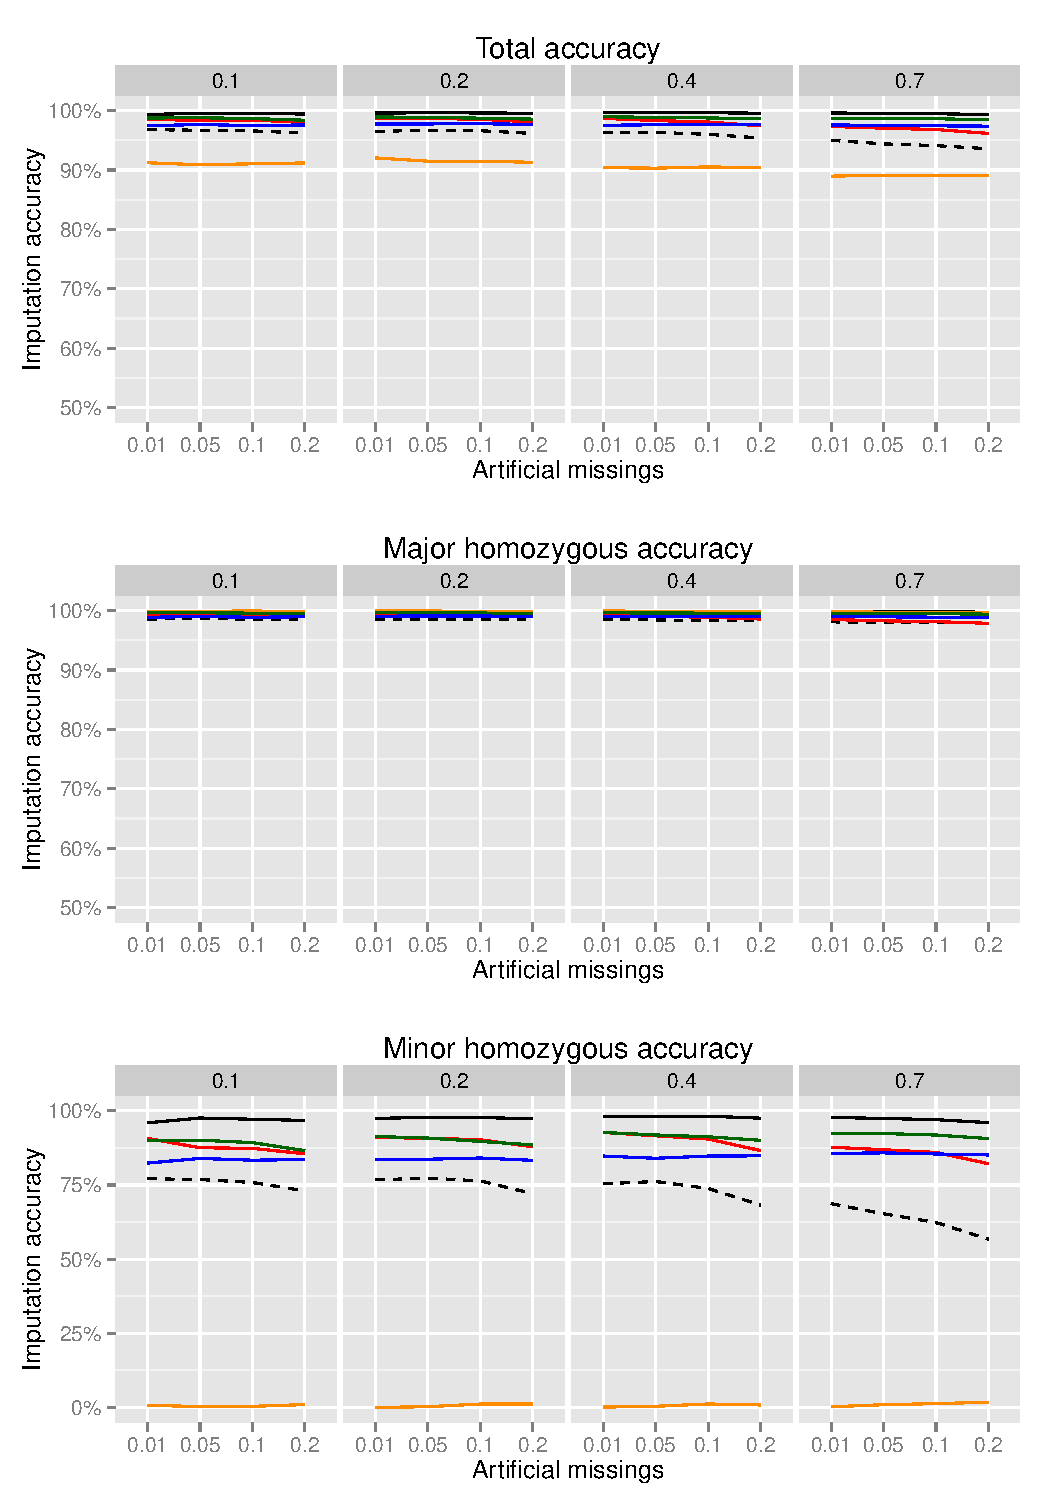
\includegraphics[width=0.95\textwidth]{SupplFig07_Rice-chrom-4.pdf}\caption{
imputation accuracies overall, for the major homozygous genotype (AA) and for the minor homozygous genotype (BB) in datasets consisting of
10\%, 20\%, 40\% and 70\% allowed missing data per locus (boxes) with 1\%, 5\%, 10\% and 20\%
additional missing values artificially introduced (x-axis) for rice chromosome 4 data.
Lines colors represent the five imputation algorithms: MNI
(orange), KNNI (red), SVDI (blue), RFI (green) and Beagle (black)}\end{figure}
\begin{figure}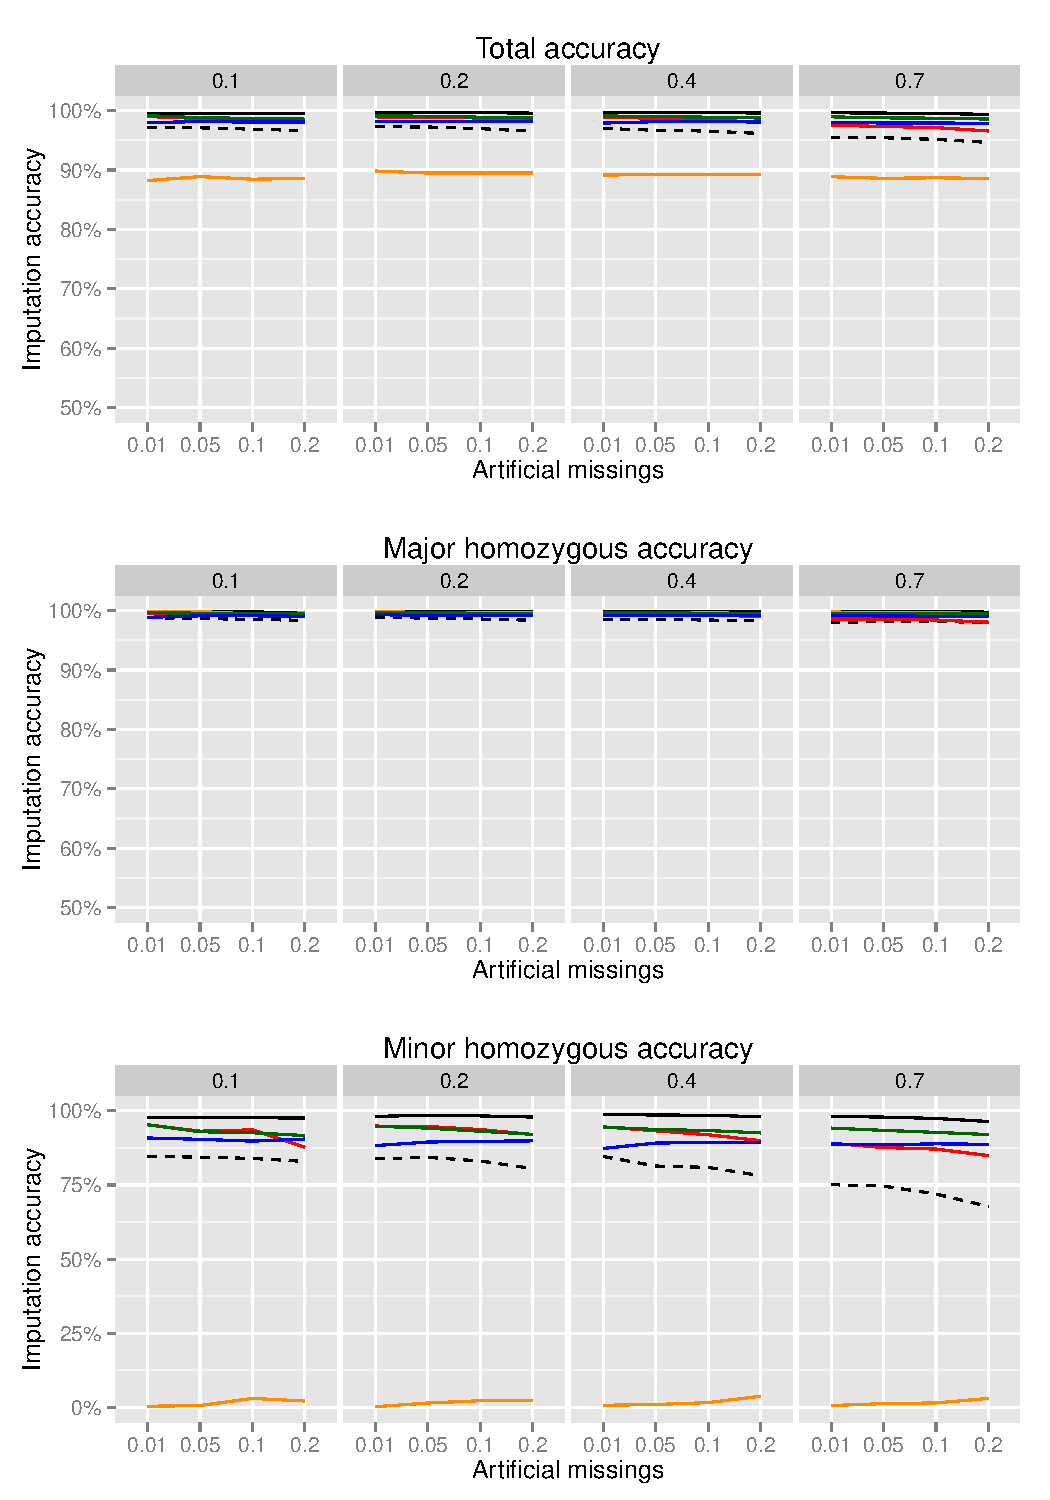
\includegraphics[width=0.95\textwidth]{SupplFig08_Rice-chrom-5.pdf}\caption{
imputation accuracies overall, for the major homozygous genotype (AA) and for the minor homozygous genotype (BB) in datasets consisting of
10\%, 20\%, 40\% and 70\% allowed missing data per locus (boxes) with 1\%, 5\%, 10\% and 20\%
additional missing values artificially introduced (x-axis) for rice chromosome 5 data.
Lines colors represent the five imputation algorithms: MNI
(orange), KNNI (red), SVDI (blue), RFI (green) and Beagle (black)}\end{figure}
\begin{figure}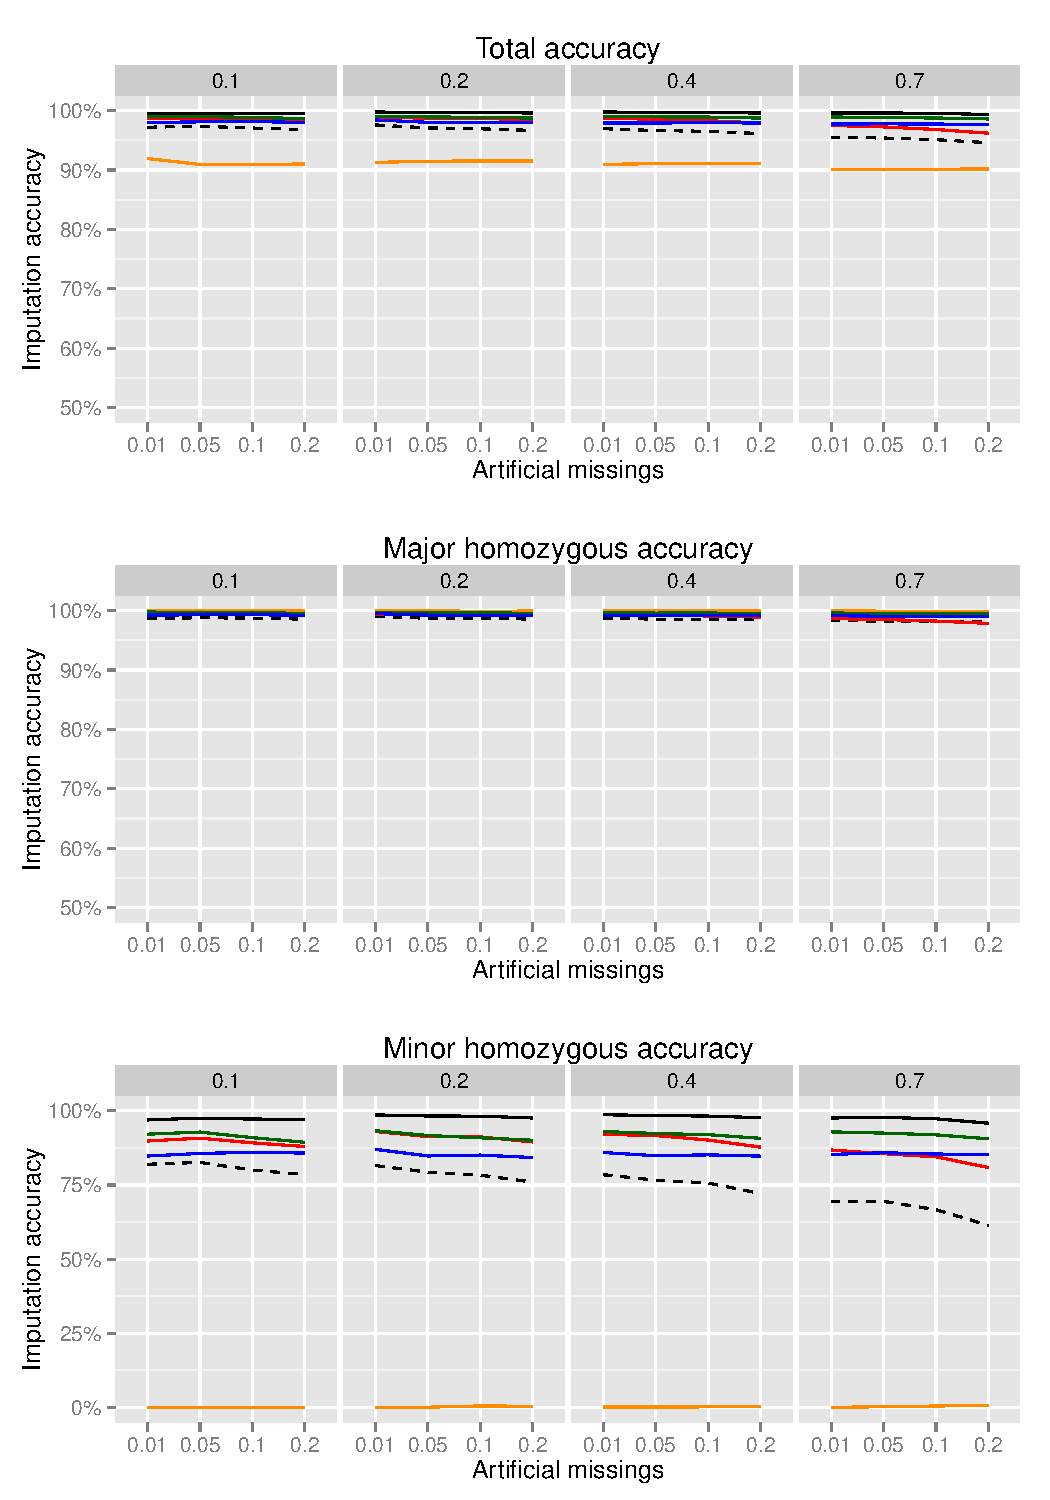
\includegraphics[width=0.95\textwidth]{SupplFig09_Rice-chrom-6.pdf}\caption{
imputation accuracies overall, for the major homozygous genotype (AA) and for the minor homozygous genotype (BB) in datasets consisting of
10\%, 20\%, 40\% and 70\% allowed missing data per locus (boxes) with 1\%, 5\%, 10\% and 20\%
additional missing values artificially introduced (x-axis) for rice chromosome 6 data.
Lines colors represent the five imputation algorithms: MNI
(orange), KNNI (red), SVDI (blue), RFI (green) and Beagle (black)}\end{figure}
\begin{figure}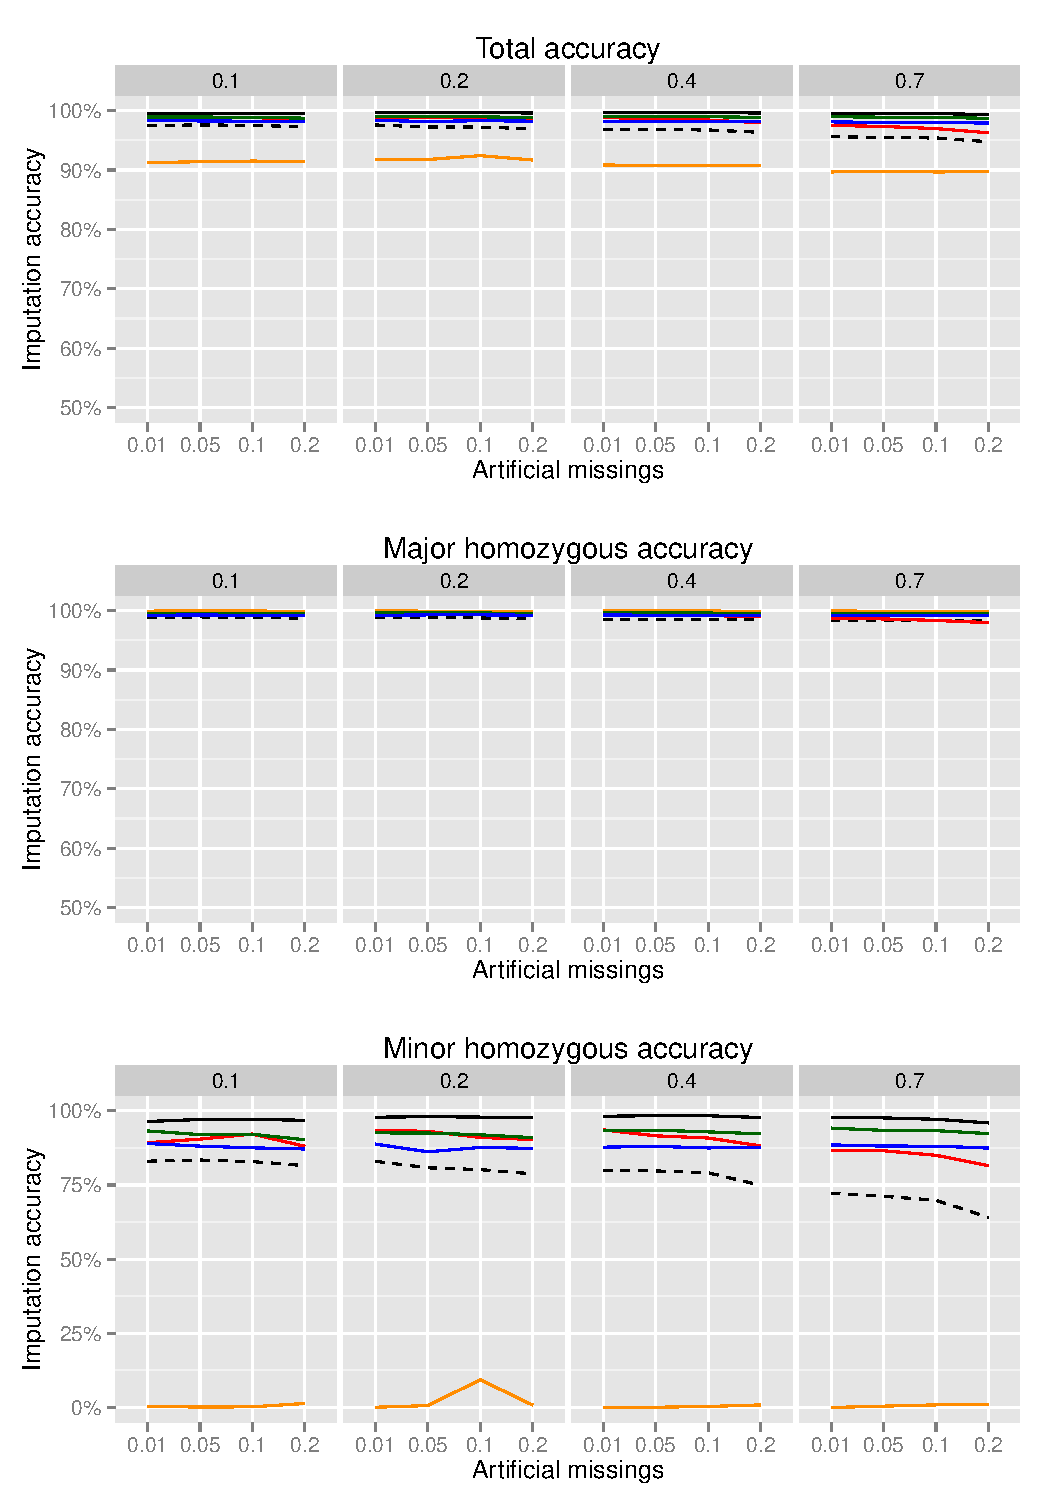
\includegraphics[width=0.95\textwidth]{SupplFig10_Rice-chrom-7.pdf}\caption{
imputation accuracies overall, for the major homozygous genotype (AA) and for the minor homozygous genotype (BB) in datasets consisting of
10\%, 20\%, 40\% and 70\% allowed missing data per locus (boxes) with 1\%, 5\%, 10\% and 20\%
additional missing values artificially introduced (x-axis) for rice chromosome 7 data.
Lines colors represent the five imputation algorithms: MNI
(orange), KNNI (red), SVDI (blue), RFI (green) and Beagle (black)}\end{figure}
\begin{figure}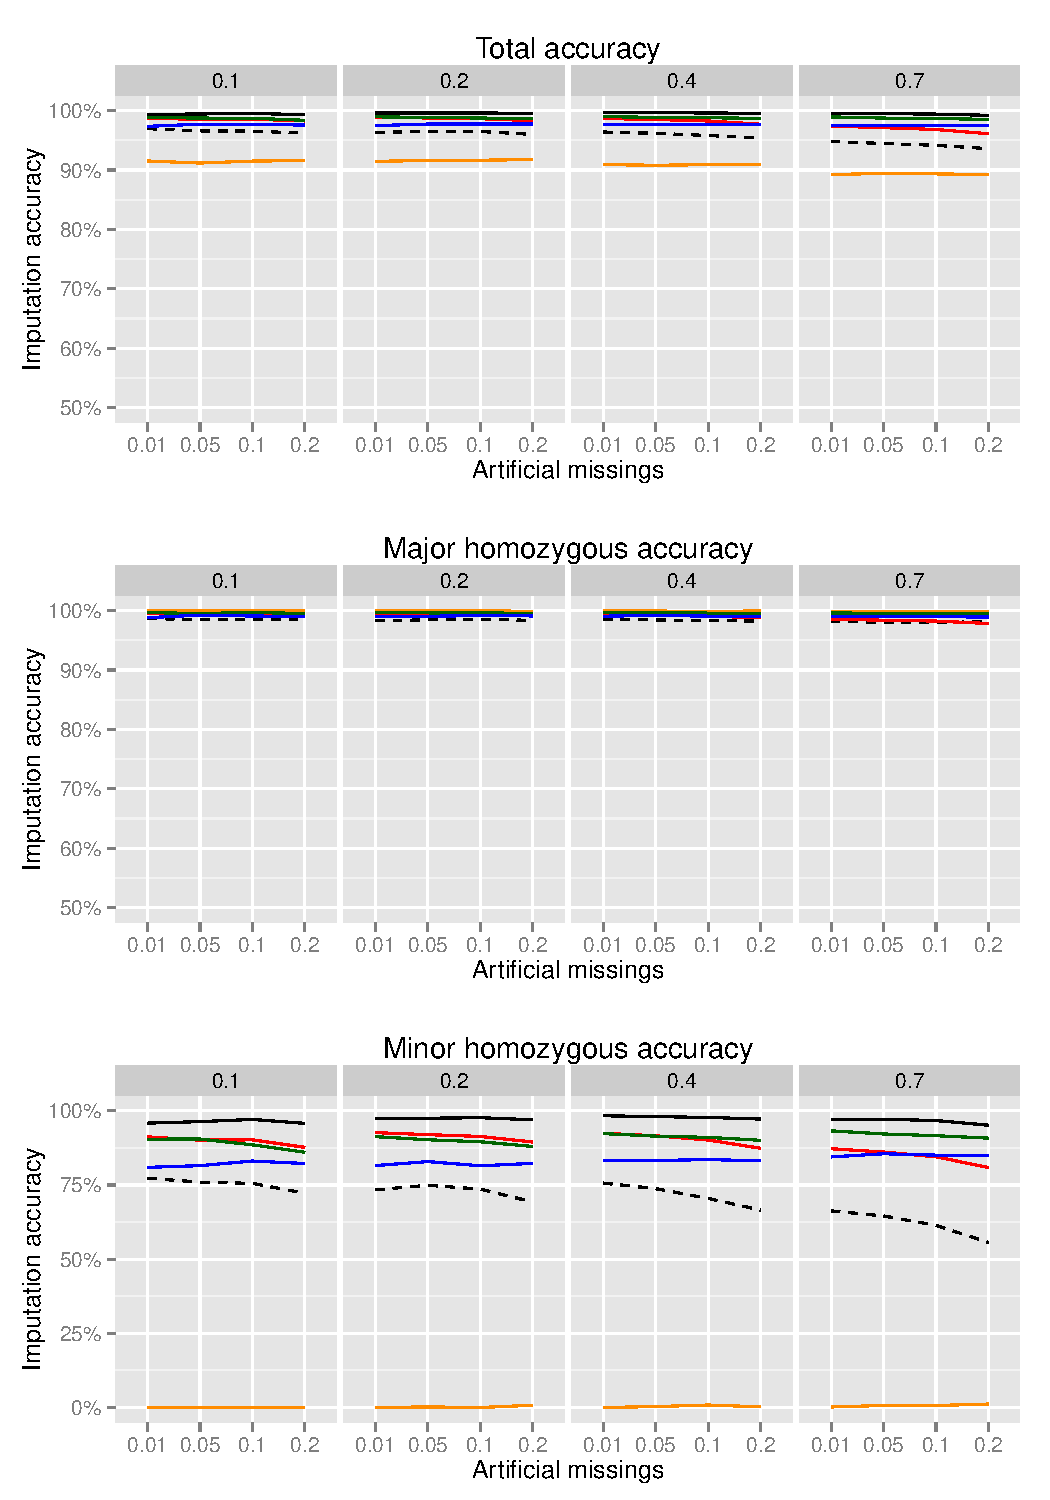
\includegraphics[width=0.95\textwidth]{SupplFig11_Rice-chrom-8.pdf}\caption{
imputation accuracies overall, for the major homozygous genotype (AA) and for the minor homozygous genotype (BB) in datasets consisting of
10\%, 20\%, 40\% and 70\% allowed missing data per locus (boxes) with 1\%, 5\%, 10\% and 20\%
additional missing values artificially introduced (x-axis) for rice chromosome 8 data.
Lines colors represent the five imputation algorithms: MNI
(orange), KNNI (red), SVDI (blue), RFI (green) and Beagle (black)}\end{figure}
\begin{figure}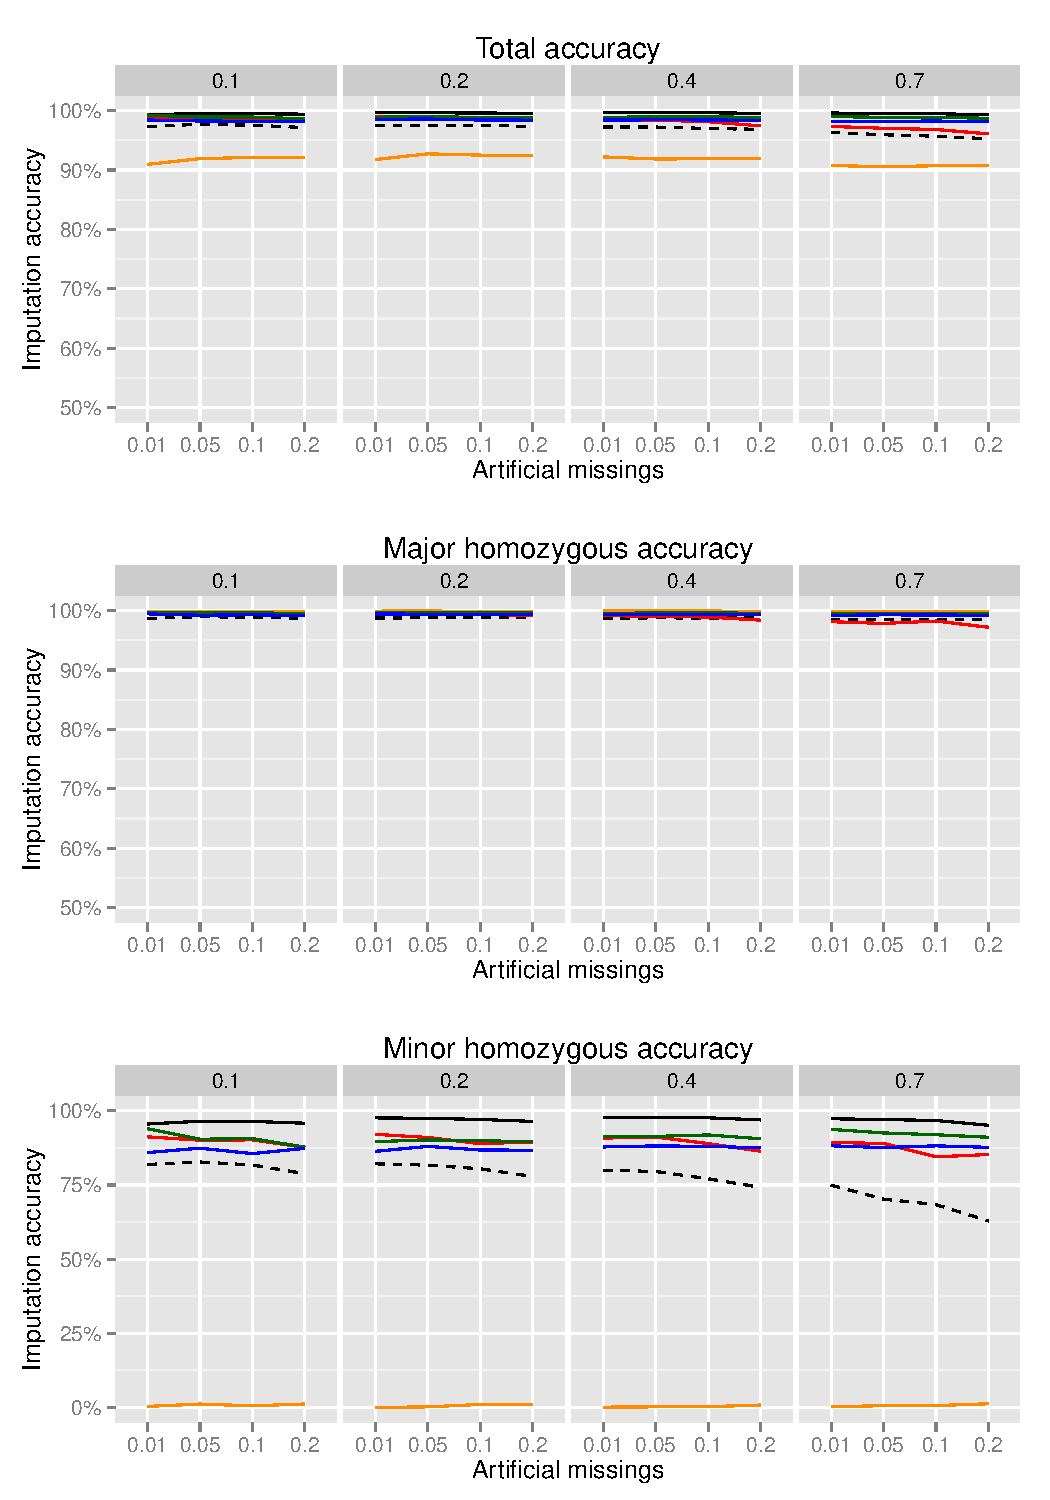
\includegraphics[width=0.95\textwidth]{SupplFig12_Rice-chrom-9.pdf}\caption{
imputation accuracies overall, for the major homozygous genotype (AA) and for the minor homozygous genotype (BB) in datasets consisting of
10\%, 20\%, 40\% and 70\% allowed missing data per locus (boxes) with 1\%, 5\%, 10\% and 20\%
additional missing values artificially introduced (x-axis) for rice chromosome 9 data.
Lines colors represent the five imputation algorithms: MNI
(orange), KNNI (red), SVDI (blue), RFI (green) and Beagle (black)}\end{figure}
\begin{figure}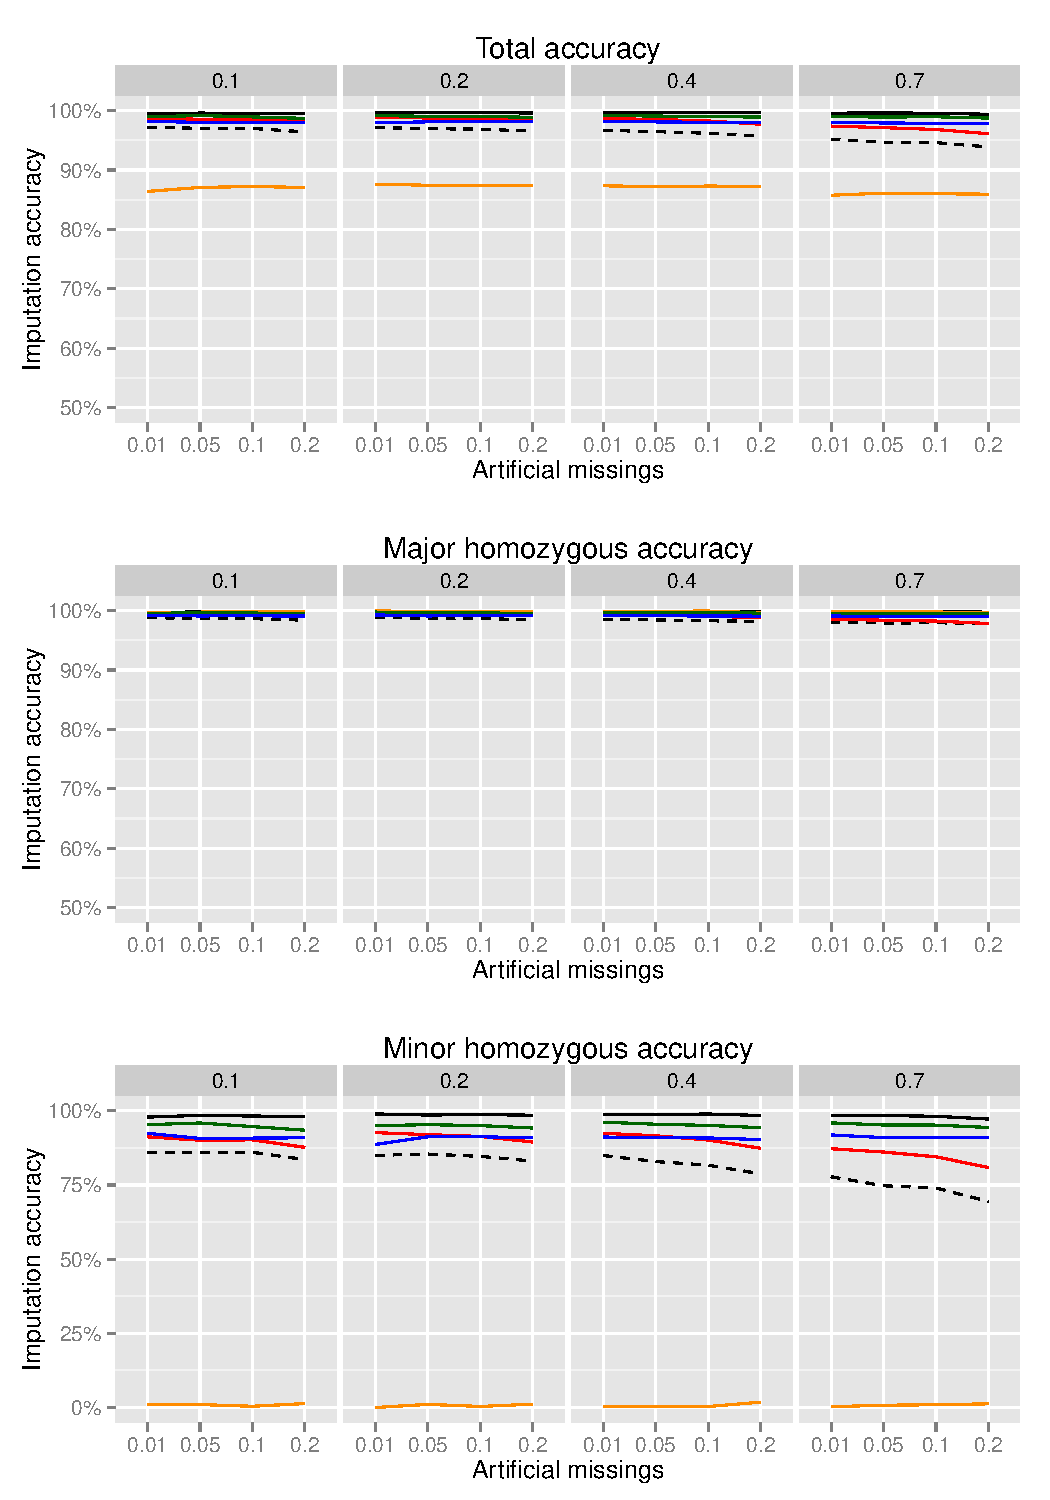
\includegraphics[width=0.95\textwidth]{SupplFig13_Rice-chrom-10.pdf}\caption{
imputation accuracies overall, for the major homozygous genotype (AA) and for the minor homozygous genotype (BB) in datasets consisting of
10\%, 20\%, 40\% and 70\% allowed missing data per locus (boxes) with 1\%, 5\%, 10\% and 20\%
additional missing values artificially introduced (x-axis) for rice chromosome 10 data.
Lines colors represent the five imputation algorithms: MNI
(orange), KNNI (red), SVDI (blue), RFI (green) and Beagle (black)}\end{figure}
\begin{figure}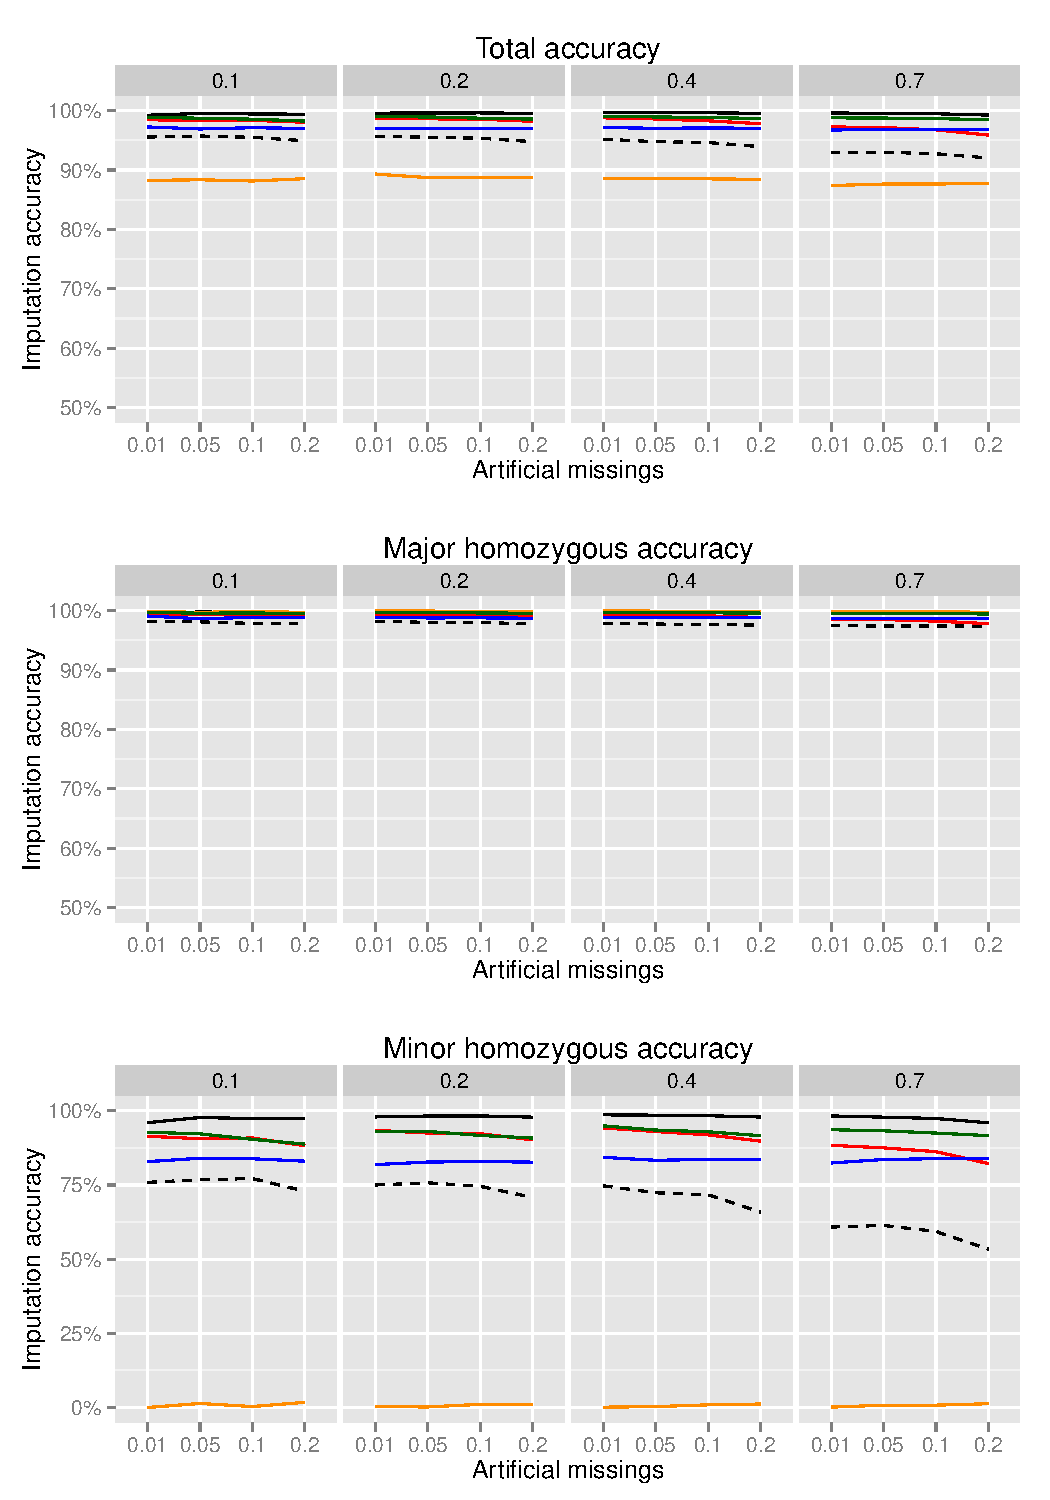
\includegraphics[width=0.95\textwidth]{SupplFig14_Rice-chrom-11.pdf}\caption{
imputation accuracies overall, for the major homozygous genotype (AA) and for the minor homozygous genotype (BB) in datasets consisting of
10\%, 20\%, 40\% and 70\% allowed missing data per locus (boxes) with 1\%, 5\%, 10\% and 20\%
additional missing values artificially introduced (x-axis) for rice chromosome 11 data.
Lines colors represent the five imputation algorithms: MNI
(orange), KNNI (red), SVDI (blue), RFI (green) and Beagle (black)}\end{figure}
\begin{figure}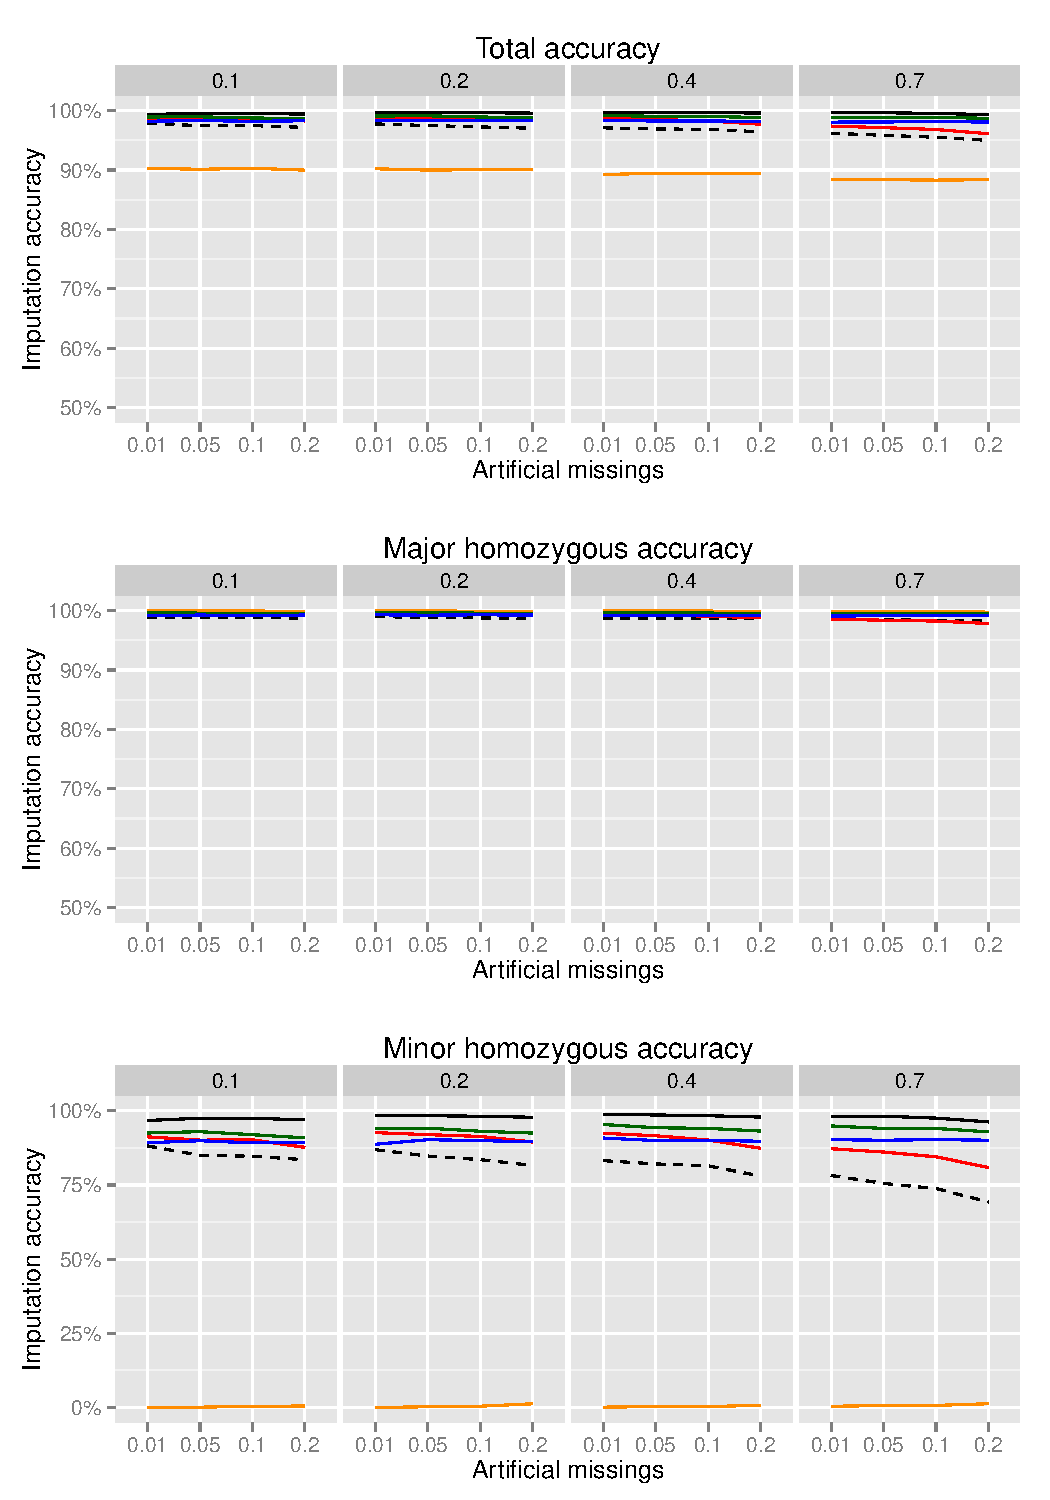
\includegraphics[width=0.95\textwidth]{SupplFig15_Rice-chrom-12.pdf}\caption{
imputation accuracies overall, for the major homozygous genotype (AA) and for the minor homozygous genotype (BB) in datasets consisting of
10\%, 20\%, 40\% and 70\% allowed missing data per locus (boxes) with 1\%, 5\%, 10\% and 20\%
additional missing values artificially introduced (x-axis) for rice chromosome 12 data.
Lines colors represent the five imputation algorithms: MNI
(orange), KNNI (red), SVDI (blue), RFI (green) and Beagle (black)}\end{figure}
\begin{figure}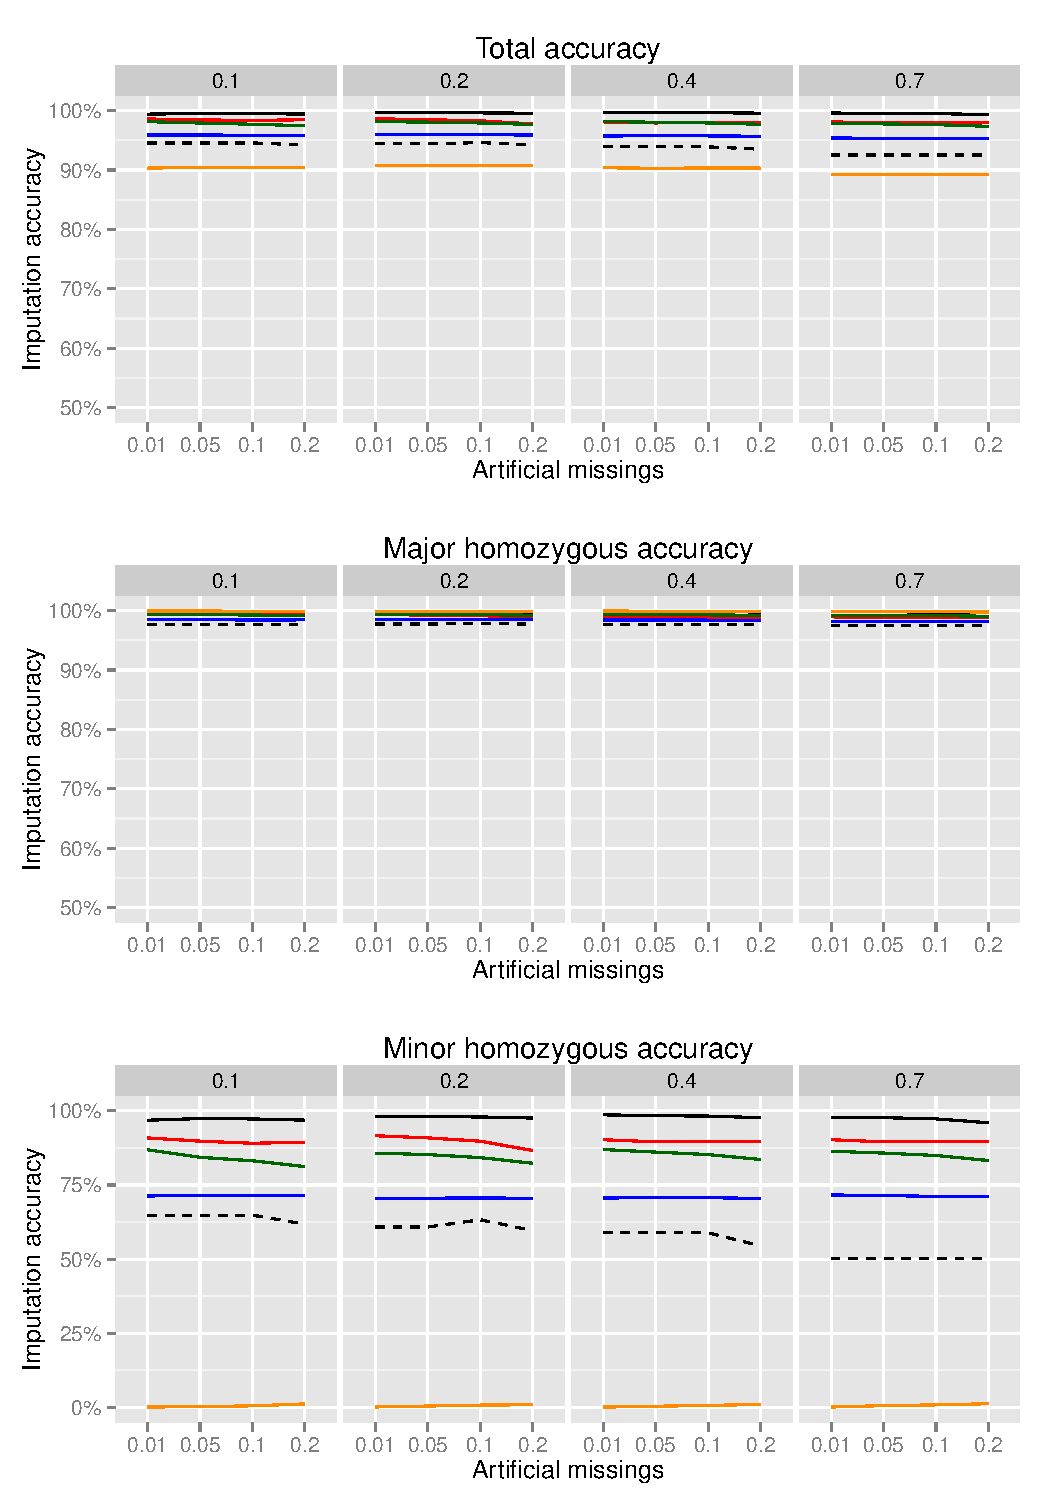
\includegraphics[width=0.95\textwidth]{SupplFig16_Rice.pdf}\caption{
imputation accuracies overall, for the major homozygous genotype (AA) and for the minor homozygous genotype (BB) in datasets consisting of
10\%, 20\%, 40\% and 70\% allowed missing data per locus (boxes) with 1\%, 5\%, 10\% and 20\%
additional missing values artificially introduced (x-axis) for whole rice data set.
Lines colors represent the five imputation algorithms: MNI
(orange), KNNI (red), SVDI (blue), RFI (green) and Beagle (black)}\end{figure}













 






% BibTeX users please use one of
%\bibliographystyle{spbasic}      % basic style, author-year citations
\bibliographystyle{spmpsci}      % mathematics and physical sciences
%\bibliographystyle{spphys}       % APS-like style for physics

%removing the whole command stops the section title to appear
%\bibliography{inputs/nazzicari.bib}   % name your BibTeX data base

\end{document}
% end of file template.tex

